\documentclass[border=8pt]{standalone}
\usepackage{tikz}
\usepackage{xcolor}
\usetikzlibrary{arrows.meta, positioning, fit, backgrounds, calc}
\definecolor{academicblue}{RGB}{30,64,105}
\definecolor{academicgray}{RGB}{100,116,139}
\definecolor{accent}{RGB}{180,120,40}
\begin{document}
\resizebox{8.4cm}{!}{%
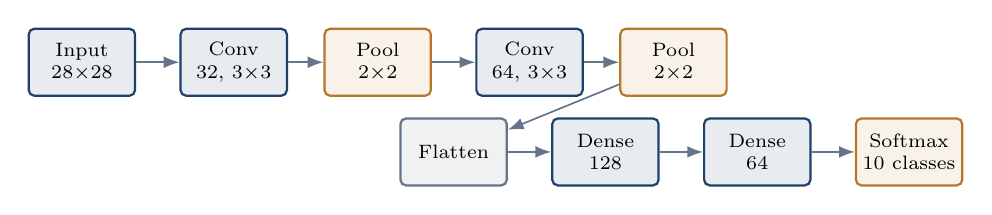
\begin{tikzpicture}[
  font=\scriptsize,
  box/.style={rectangle, rounded corners=2pt, draw=#1, line width=0.8pt,
    fill=#1!10, minimum width=1.35cm, minimum height=0.85cm, align=center, inner sep=2pt},
  pool/.style={box=accent},
  arr/.style={-{Latex[length=2mm]}, draw=academicgray, line width=0.6pt}
]
\node[box=academicblue] (in) {Input\\28$\times$28};
\node[box=academicblue, right=0.55cm of in] (c1) {Conv\\32, 3$\times$3};
\node[pool, right=0.45cm of c1] (p1) {Pool\\2$\times$2};
\node[box=academicblue, right=0.55cm of p1] (c2) {Conv\\64, 3$\times$3};
\node[pool, right=0.45cm of c2] (p2) {Pool\\2$\times$2};
\node[box=academicgray, below=0.7cm of $(c1)!0.5!(p2)$] (flat) {Flatten};
\node[box=academicblue, right=0.55cm of flat] (d1) {Dense\\128};
\node[box=academicblue, right=0.55cm of d1] (d2) {Dense\\64};
\node[box=accent, right=0.55cm of d2] (out) {Softmax\\10 classes};
\draw[arr] (in)--(c1); \draw[arr] (c1)--(p1); \draw[arr] (p1)--(c2);
\draw[arr] (c2)--(p2); \draw[arr] (p2)--(flat);
\draw[arr] (flat)--(d1); \draw[arr] (d1)--(d2); \draw[arr] (d2)--(out);
\end{tikzpicture}%
}
\end{document}
